
\documentclass[12pt,a4paper]{article}
\usepackage{setspace}
%\doublespacing

\usepackage{geometry}
\geometry{legalpaper, margin=1in}

\usepackage[T1]{fontenc}
\usepackage[bitstream-charter]{mathdesign}

\usepackage[latin1]{inputenc}							% Input encoding
\usepackage{amsmath}									% Math

\usepackage{xcolor}
\definecolor{bl}{rgb}{0.1,0.1,0.3} 

\usepackage{sectsty}
\usepackage[compact]{titlesec} 
\allsectionsfont{\color{bl}\scshape\selectfont}

%customary definitons..
\allowdisplaybreaks
\usepackage{algorithm}
\usepackage{algorithmic}
\usepackage{mathtools}
\usepackage{graphicx}
\usepackage{float}

%%%%% Definitions
% Define a new command that prints the title only
\makeatletter							% Begin definition
\def\printtitle{%						% Define command: \printtitle
    {\color{bl} \centering \huge \sc \textbf{\@title}\par}}		% Typesetting
\makeatother							% End definition

\title{Stochastic Multi-Products Order-Redistribution Problem.\\ }

% Define a new command that prints the author(s) only
\makeatletter							% Begin definition
\def\printauthor{%					% Define command: \printauthor
    {\centering \small \@author}}				% Typesetting
\makeatother							% End definition

\author{%
	Sanchit Singh \\
	sanchit@vt.edu \\
	\vspace{20pt}
	}

% Custom headers and footers
\usepackage{fancyhdr}
	\pagestyle{fancy}					% Enabling the custom headers/footers
\usepackage{lastpage}	
	% Header (empty)
	\lhead{}
	\chead{}
	\rhead{}
	% Footer (you may change this to your own needs)
	\lfoot{\footnotesize}
	\cfoot{}
	\rfoot{\footnotesize page \thepage\ of \pageref{LastPage}}	% "Page 1 of 2"
	\renewcommand{\headrulewidth}{0.0pt}
	\renewcommand{\footrulewidth}{0.4pt}

% Change the abstract environment
\usepackage[runin]{abstract}			% runin option for a run-in title
\setlength\absleftindent{10pt}		% left margin
\setlength\absrightindent{10pt}		% right margin
\abslabeldelim{\quad}						% 
\setlength{\abstitleskip}{-10pt}
\renewcommand{\abstractname}{}
\renewcommand{\abstracttextfont}{\color{bl} \small \slshape}	% slanted text


%%% Start of the document
\begin{document}
%%% Top of the page: Author, Title and Abstact

\printtitle 

\printauthor

\begin{abstract}
We address a commonly observed scenario in a supply chain of some company wherein the company operates a set of warehouses or distribution centers (DCs) located in different geographical locations. Each DC has a recurring demand for a set of products in a multi-period time horizon, and a demand for any one product in any time period is stochastic and scenario based. Demands have to be met at a DC within that time-period after they are realized. From the view point of any DC, we  consider three types of suppliers; one-primary suppliers that are located in far off places like international suppliers, two-primary suppliers that can be considered domestic and are nearby, and, three-secondary suppliers like other DCs (under the same company) which can used as transfer points or inventory buffers. \\
Usually, one overlooks the importance of secondary suppliers in meeting shortfall of demands, but this case deserves attention, especially when a shortfall of demands occurs (owing to prior decisions) and can not be met from primary suppliers in short time spans. Therefore, in this study, we consider the first and third type of suppliers, as mentioned above. The primary supplier located far off can be requested to send a shipment in fixed time (although relatively large) to its receiving DC. For sake of convenience, we assume that only one supplier can make a single shipment in any one time period to a DC, although the primary supplier can still supply an assortment of products in that shipment. The decisions made here (we call this as "order phase") are how much to order for each product (under certain constraints), that the supplier provides, and in which time periods. Since the demand for each product at its corresponding DC in various time periods are stochastic, the system is allowed to make recourse decisions, after any particular product's demand realization at some DC. This brings us to the role of secondary suppliers, i.e. few DCs serve as suppliers for certain products to others, with such re-routing of products to be accomplished within one time-period. The decisions made here (we call this as "redistribution phase") are what quantity of pickup or delivery does the DCs require for any product and how to plan routes for in-house fleet of vehicles to serve these in a constrained manner. The second part of decisions in any time period are closely related to another problem in transportation known as \emph{Pickup and Delivery Vehicle Routing Problems with Time Windows} (PDVRPTW). \\
There are some variations which can be easily integrated within our model, making the problem more realistic from a company's viewpoint, at the same time more intractable. Therefore, we shall discount these variations in our current study, and keep them aside for future study. We will discuss these here in brief. (i) Accounting for one or more of transfer points might either be a necessary condition (like in multi-modal transportation), or even if not, a better strategy in PDVRPTW. (ii) Multiple shipments could be arriving at any DC from various suppliers in any one time period. (iii) The company might be using its own fleet of vehicles for transportation of some of the products form its primary suppliers which are domestic. In that case, vehicles can be used not just for internal redistribution between DCs, but also for transportation of products from external primary suppliers located domestically. (iv) Note that, we have considered that all products arriving at various DCs are ready made ones, which are bought as it is, without consideration for their assembly (serial, parallel or mix of both) or related activities as is common in make-to-assemble or just-in-time systems. This will introduce additional complexity in the problem since the product specific processes will also have to be monitored, which may or may not be under the company's control, but none the less such integration will bring us closer to actual requirements in the industry and give us an opportunity to implement philosophies such as lot-streaming or deploying multiple sourcing for a product etc in a meaningful way.
\end{abstract}
\underline{Fundamental sets}: \\
$\textbf{I}$ \quad = \{1,2,\ldots ,|\textbf{I}|\}, set of products \\
$\textbf{J}$ \quad = \{1,2,\ldots ,|\textbf{J}|\}, set of DCs \\
$\textbf{T}$ \quad = \{1,2,\ldots ,|\textbf{T}|\}, set of time periods \\
$\textbf{V}$ \quad = \{1,2,\ldots ,|\textbf{V}|\}, set of vehicles operating in each time period \\
$(i,\bar{t},j)\in \textbf{ITJ}$ \quad = set of triplets, representing whether product $i$ can be shipped to DC $j$ in time period $\bar{t}$ $(1\leq \bar{t} \leq |\textbf{T}|-1)$, from its primary supplier \\
\underline{Shipping from primary suppliers related}: \\
$lt_{i,\bar{t}}^{j}$ \quad lead time for shipment indexed as $(i,\bar{t},j)\in \textbf{ITJ}$ such that it arrives at the DC $j$ at the start of time period $\bar{t}+lt_{i,\bar{t}}^{j}$, $lt_{i,\bar{t}}^{j}\geq 1$, and $\bar{t}+lt_{i,\bar{t}}^{j}\leq |\textbf{T}|, \forall (i,\bar{t},j)\in \textbf{ITJ}$\\
$sfc_{\bar{t}}^{j}$ \quad fixed cost to make a shipment (of various products) to DC $j$ in time period $\bar{t}$ such that, $\forall (i,\bar{t},j)\in \textbf{ITJ}$ \\
$svc_{i,\bar{t}}^{j}$ \quad cost per unit volume for shipping product $i$ to DC $j$ in time period $\bar{t}$ such that, $\forall (i,\bar{t},j)\in \textbf{ITJ}$\\
$svu_{i}^{j}$ \quad shipping volume utilization per unit of product $i$ (same in any time period) to DC $j$ such that, $\forall (i,\bar{t},j)\in \textbf{ITJ}$\\
$svm_{i,\bar{t}}^{j}$ \quad shipping maximum volume allowed for product $i$ in time period $\bar{t}$ to DC $j$ such that, $\forall (i,\bar{t},j)\in \textbf{ITJ}$\\
$\widehat{svm}_{\bar{t}}^{j}$ \quad shipping maximum volume allowed for all products in time period $\bar{t}$ to DC $j$ such that, $\forall (i,\bar{t},j)\in \textbf{ITJ}$\\
$swc_{i,\bar{t}}^{j}$ \quad cost per unit weight for shipping product $i$ to DC $j$  in time period $\bar{t}$ such that, $\forall (i,\bar{t},j)\in \textbf{ITJ}$\\
$swu_{i}^{j}$ \quad shipping weight utilization per unit of product $i$ (same in any time period) to DC $j$ such that, $\forall (i,\bar{t},j)\in \textbf{ITJ}$\\
$swm_{i,\bar{t}}^{j}$ \quad shipping maximum weight allowed for product $i$ in time period $\bar{t}$ to DC $j$ such that, $\forall (i,\bar{t},j)\in \textbf{ITJ}$\\
$\widehat{swm}_{\bar{t}}^{j}$ \quad shipping maximum weight allowed for all products in time period $\bar{t}$ to DC $j$ such that, $\forall (i,\bar{t},j)\in \textbf{ITJ}$\\
$d_{i,t}^{j}$ \quad demand (zero or positive) of product $i$ at DC $j$ in time period $t$ $(t\geq 2)$ \\
$dlc_{i,t}^{j}$ \quad cost for incurring the demand loss of a unit of product $i$ at DC $j$ in time period $t$ $(t\geq 2)$ \\
\underline{Inventory at DCs related}: \\
$ivc_{i,t}^{j}$ \quad inventory cost to carry unit volume of product $i$ from time period $t$ to $t+1$ for DC $j$ \\
$ivu_{i}^{j}$ \quad inventory volume utilization per unit of product $i$ (same in any time period) for DC $j$ \\
$ivm_{i,t}^{j}$ \quad inventory maximum volume allowed for product $i$ in time period $t$ for DC $j$ \\
$\widehat{ivm}_{t}^{j}$ \quad inventory maximum volume allowed for all products in time period $t$ for DC $j$ \\
\underline{Transportation among DCs (PDVRP) related}: \\
\textbf{P} \quad = \{1,2,\ldots ,$n$\}, set of pickup nodes, $n$ = |\textbf{J}|*|\textbf{I}|*(|\textbf{J}|-1) \\
\textbf{D} \quad = \{$n$+1,$n$+2,\ldots ,2$n$\}, set of delivery nodes \\
\textbf{O} \quad = \{2$n$+1,2$n$+2,\ldots ,$2n+|\textbf{V}|$\}, set of nodes representing depots for vehicles \\
\textbf{N} \quad = \textbf{P} $\cup$ \textbf{D} $\cup$ \textbf{O} \\
\textbf{A} \quad = \textbf{N} $\times$ \textbf{N}, set of arcs connecting different nodes in \textbf{N}, ($(j,j)\not \in \textbf{A}\colon j\in \textbf{N}$) \\
$vvu_{v}^{k}$ \quad volume utilization on vehicle $v$ by a unit of the product that is picked (or dropped) at node $k\in \textbf{N}$ \\
\text{ } \quad \qquad (note that only a unique product (or none) is assigned to be either picked up or dropped at any node $k\in \textbf{N}$)\\
$tfc_{v}$ \quad fixed transportation cost incurred if vehicle $v$ is operated in a time period \\
$tvc_{v}^{jk}$ \quad variable transportation cost to carry a unit volume of (mix of) products, if vehicle $v$ travels on arc $(j,k) \in \textbf{A}$
$t_{v}^{j,k}$ \quad travel time on arc $(j,k)\in \textbf{A}$ for vehicle $v$ \\
$st_{v}^{j}$ \quad fixed service time required to load or unload a vehicle $v$ at node $k\in \textbf{N}$ ($st_{v}^{j}=0, \forall j \in \textbf{O}, \forall v \in \textbf{V} $) \\
$\epsilon_v$ \quad minimum pickup quantity required from any node by vehicle $v \in \textbf{V}$ \\
$q_v$ \quad maximum vehicle capacity $v \in \textbf{V}$ \\
$\tau$ \quad time length of any one period \\
\underline{Variables}: \\
All the variables are represented in upper case, and the parameters in lower case. \\
$
\begin{matrix*}[l]
P_{i,\bar{t},t}^{j} & \forall (i,\bar{t},j)\in \textbf{ITJ}, \forall t \in \textbf{T} 
& \parbox[t]{0.65\linewidth}{Units of product $i$ ordered in period $\bar{t}$ and available at DC $j$ at the start of period $t$}\\
Z_{\bar{t}}^{j} &  \forall (i,\bar{t},j)\in \textbf{ITJ} 
& \parbox[t]{0.65\linewidth}{Binary variable indicating whether a shipment was ordered for DC $j$ in time period $\bar{t}$ or not} \\
D_{1,i,t}^{j{}} &  \forall i \in \textbf{I}, \forall j \in \textbf{J}, \forall t \in \textbf{T} 
& \parbox[t]{0.65\linewidth}{Units of product $i$ in current inventory at the start of period $t$, after its demand has been met by the inventory from the last period and/or direct shipments from various suppliers} \\
D_{i,t}^{j{'}}  & \forall i \in \textbf{I}, \forall j \in \textbf{J}, \forall t \in \textbf{T} 
& \parbox[t]{0.65\linewidth}{Demand shortage for product $i$ that is met from redistribution of inventory among DCs, by the end of the same time period in which the demand was realized}\\
L_{i,t}^{j{+}}  & \forall i \in \textbf{I}, \forall j \in \textbf{J}, \forall t \in \textbf{T} 
& \parbox[t]{0.65\linewidth}{Units of product $i$ sent to other DCs from DC $j$ in time period $t$} \\
U_{i,t}^{j{+}} & \forall i \in \textbf{I}, \forall j \in \textbf{J}, \forall t \in \textbf{T} & 
\parbox[t]{0.65\linewidth}{Binary variable, set to unity if $L_{i,t}^{j{+}}$ is positive}\\
D_{2,i,t}^{j} & \forall i \in \textbf{I}, \forall j \in \textbf{J}, \forall t \in \textbf{T} & 
\parbox[t]{0.65\linewidth}{Units of product $i$ left in current inventory after some of it has been sent to other DCs} \\
L_{i,t}^{j{-}} & \forall i \in \textbf{I}, \forall j \in \textbf{J}, \forall t \in \textbf{T} & 
\parbox[t]{0.65\linewidth}{Units of product $i$ coming to DC $j$ from other DCs, by the end of time period $t$} \\
U_{i,t}^{j{-}} & \forall i \in \textbf{I}, \forall j \in \textbf{J}, \forall t \in \textbf{T}
& \parbox[t]{0.65\linewidth}{Binary variable, set to unity if $L_{i,t}^{j{-}}$ is positive (To make the model more realistic, in any time period, material can either be shipped from a DC to other DCs - when there is excess of it at the start of the time period, or received by a DC from other DCs - when it needs to increase its own inventory or fulfill any shortfall of current period demand, but not both) }\\
D_{3,i,t}^{j} & \forall i \in \textbf{I}, \forall j \in \textbf{J}, \forall t \in \textbf{T} & 
\parbox[t]{0.65\linewidth}{Units of product $i$ in current inventory after some of it has been received from other DCs} \\
D_{i,t}^{j{''}} & \forall i \in \textbf{I}, \forall j \in \textbf{J}, \forall t \in \textbf{T} & 
\parbox[t]{0.65\linewidth}{Lost demand for product $i$ that could not be met even in the "redistribution phase" (Fulfilling of shortfall of demand from future is not considered in the model)}\\
S_{i,t}^{j} & \forall i \in \textbf{I}, \forall j \in \textbf{J}, \forall t \in \textbf{T} 
& \parbox[t]{0.65\linewidth}{inventory of product $i$ at DC $j$, at the end of time period $t$ that is carried over to next time period (Note that initial inventories i.e. $S_{i,0}^{j}$ could be zero or positive, and is specified as a parameter. Also, stocking of inventory at any DC, at the end of a time period, is not allowed at the expense of lost demand for any product)} \\
L_{i,t}^{j,k{+}} & \forall i \in \textbf{I}, \forall j,k \in \textbf{J}, j\neq k, \forall t \in \textbf{T} 
& \parbox[t]{0.65\linewidth}{Units of product $i$ sent to DC $k$ from DC $j$ in time period $t$} \\
L_{i,t}^{j,k{-}} & \forall i \in \textbf{I}, \forall j,k \in \textbf{J}, j\neq k, \forall t \in \textbf{T} 
& \parbox[t]{0.65\linewidth}{Units of product $i$ received by DC $j$ from DC $k$ in time period $t$} \\
Y_{v,t}^{k} & \forall v \in \textbf{V}, \forall k \in \textbf{N}, \forall t \in \textbf{T}
& \parbox[t]{0.65\linewidth}{Binary variable, set to unity if vehicle $v$ covers node $k$ in time period $t$, zero otherwise} \\
X_{v,t}^{j,k} & \forall v \in \textbf{V}, \forall (j,k) \in \textbf{A}, \forall t \in \textbf{T} 
& \parbox[t]{0.65\linewidth}{Binary variable, set to unity if vehicle $v$ covers arc $(j,k)$ in time period $t$, zero otherwise} \\
T_{v,t}^{k} & \forall v \in \textbf{V}, \forall k \in \textbf{N}, \forall t \in \textbf{T} 
& \parbox[t]{0.65\linewidth}{Time status at node $k$, by vehicle $v$ in time period $t$} \\
L_{r}^{t} & \forall r \in \textbf{P} \cup \textbf{D} , \forall (j,k) \in \textbf{A}, \forall t \in \textbf{T} 
& \parbox[t]{0.65\linewidth}{Units of a (corresponding) product to be either picked up from (if positive) or dropped at (if negative) node $r$ in time period $t$} \\
V_{v,t}^{k} & \forall v \in \textbf{V}, \forall k \in \textbf{N}, \forall t \in \textbf{T} 
& \parbox[t]{0.65\linewidth}{Capacity status (in volume) of vehicle $v$ at node $k$, in time period $t$} \\
W_{v,t}^{j,k} & \forall v \in \textbf{V}, \forall (j,k) \in \textbf{A}, \forall t \in \textbf{T}  
& \parbox[t]{0.65\linewidth}{$=V_{v,t}^{k}\times X_{v,t}^{j,k}$}
\end{matrix*}
$ \\ \\
Some understanding of variables above can be made from Figure \ref{fig:product_i_timeperiod_t}. 
\begin{figure}[H]
\centering
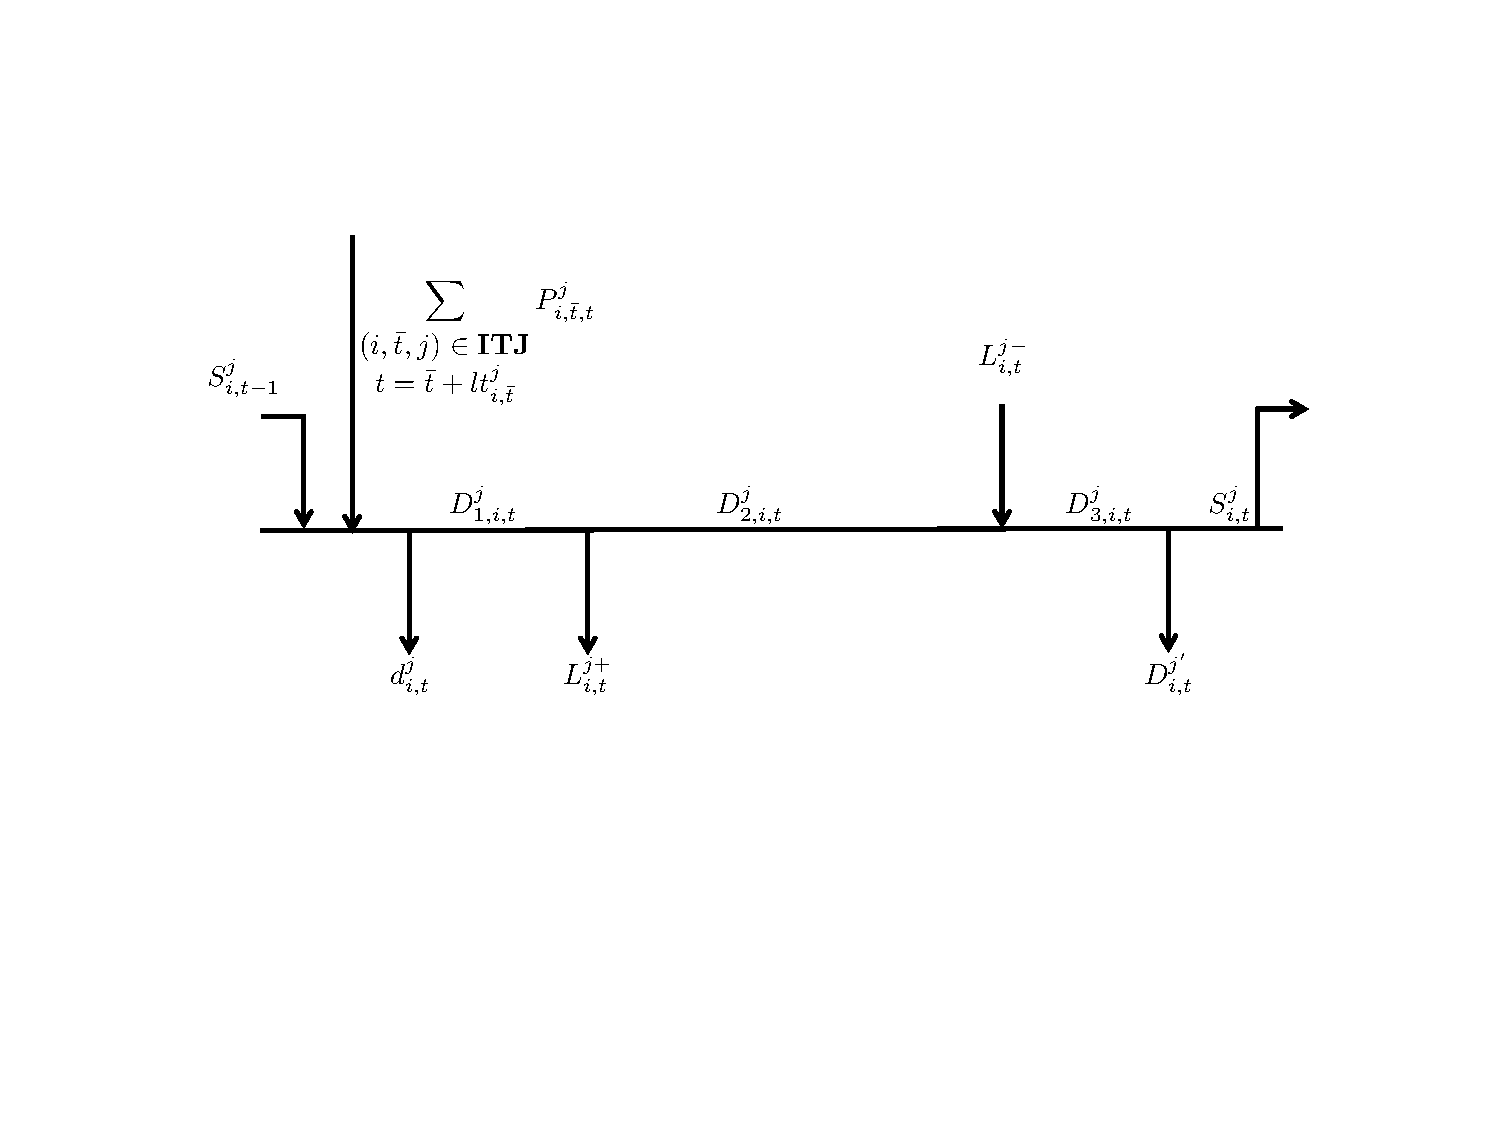
\includegraphics[trim=1cm 7cm 3cm 4cm, clip=true, totalheight=0.2\textheight]{Fig1.pdf}
\caption{Change in inventory of product $i$ in time period $t$ for DC $j$}
\label{fig:product_i_timeperiod_t}
\end{figure}

MILP model, \textbf{M1}: \\
\begin{align*}
\text{min } & \sum_{
\begin{matrix}
j\in \textbf{J},\bar{t} \in \textbf{T}, \\
\exists (i,\bar{t},j) \in \textbf{ITJ}
\end{matrix}
} sfc_{\bar{t}}^{j}Z_{\bar{t}}^{j} + \sum_{(i,\bar{t},j) \in \textbf{ITJ}} (svc_{i,\bar{t}}^{j} svu_{i,\bar{t}}^{j} +swc_{i,\bar{t}}^{j} swu_{i,\bar{t}}^{j}) P_{i,\bar{t},\bar{t}}^{j} +\sum_{i\in \textbf{I}, j\in \textbf{J}, t \in \textbf{T}} (dlc_{i,t}^{j} D_{i,t}^{j{''}} + ivc_{i,t}^{j} ivu_{i,t}^{j} S_{i,t}^{j}) \\
& + \sum_{t\in \textbf{T}, v\in \textbf{V}} tfc_{v} Y_{v,t}^{2n+v} + \sum_{t\in \textbf{T}, v\in \textbf{V}, j \in \textbf{J}, (j,k) \in \textbf{A}} tvc_{v}^{j,k} W_{v,t}^{j,k}
\end{align*}
\begin{align}
P_{i,\bar{t},t}^{j} & = 0 && \quad \forall 1\leq t\leq \bar{t}-1, \forall \bar{t}+lt_{i,\bar{t}}^{j}+1 \leq t \leq |\textbf{T}|, \nonumber\\
& && \quad \forall (i,\bar{t},j)\in \textbf{ITJ} \\
P_{i,\bar{t},t}^{j} & = P_{i,\bar{t},t-1} && \quad \forall \bar{t}+1\leq t\leq \bar{t}+lt_{i,\bar{t}}^{j}, \forall (i,\bar{t},j)\in \textbf{ITJ} \\
svu_{i,\bar{t}}^{j}P_{i,\bar{t},\bar{t}}^{j} & \leq svm_{i,\bar{t}}^{j} && \quad \forall (i,\bar{t},j)\in \textbf{ITJ} \\
\sum_{(i,\bar{t},j)\in \textbf{ITJ} } svu_{i,\bar{t}}^{j}P_{i,\bar{t},\bar{t}}^{j} & \leq \widehat{svm}_{\bar{t}}^{j} && \quad \forall j\in \textbf{J}, \forall \bar{t} \in \textbf{T} \\
swu_{i,\bar{t}}^{j}P_{i,\bar{t},\bar{t}}^{j} & \leq swm_{i,\bar{t}}^{j} && \quad \forall (i,\bar{t},j)\in \textbf{ITJ} \\
\sum_{(i,\bar{t},j)\in \textbf{ITJ} } swu_{i,\bar{t}}^{j}P_{i,\bar{t},\bar{t}}^{j} & \leq \widehat{swm}_{\bar{t}}^{j} && \quad \forall j\in \textbf{J}, \forall \bar{t} \in \textbf{T} \\
P_{i,\bar{t},\bar{t}}^{j} & \leq M Z_{\bar{t}}^{j} && \quad \forall (i,\bar{t},j)\in \textbf{ITJ} \\
& \text{where } M \text{ is a big number} && \nonumber \\
D_{0,i,t}^{j} & = S_{i,t-1}^{j}+\sum_{
\begin{matrix} 
(i,\bar{t},j)\in \textbf{ITJ} \\
t=\bar{t}+lt_{i,\bar{t}}^{j}
\end{matrix}
}
P_{i,\bar{t},t}^{j} && \quad \forall i\in \textbf{I},\forall j\in \textbf{J}, \forall t \in \textbf{T} \\
D_{1,i,t}^{j} & = \max(D_{0,i,t}^{j}-d_{i,t}^{j},0) && \quad \forall i\in \textbf{I},\forall j\in \textbf{J}, \forall t \in \textbf{T} \label{eq:max1} \\
D_{2,i,t}^{j} & = D_{1,i,t}^{j}- L_{i,t}^{j{+}} && \quad \forall i\in \textbf{I},\forall j\in \textbf{J}, \forall t \in \textbf{T} \\
D_{3,i,t}^{j} & = D_{2,i,t}^{j}+ L_{i,t}^{j{-}} && \quad \forall i\in \textbf{I},\forall j\in \textbf{J}, \forall t \in \textbf{T} \\
D_{i,t}^{j{'}} & = \max(d_{i,t}^{j}-D_{0,i,t}^{j},0) && \quad \forall i\in \textbf{I},\forall j\in \textbf{J}, \forall t \in \textbf{T} \label{eq:max2}\\
D_{i,t}^{j{''}} & = \max(D_{i,t}^{j{'}}-D_{3,i,t}^{j},0) && \quad \forall i\in \textbf{I},\forall j\in \textbf{J}, \forall t \in \textbf{T} \label{eq:max3}\\
S_{i,t}^{j} & = \max(D_{3,i,t}^{j}-D_{i,t}^{j{'}},0) && \quad \forall i\in \textbf{I},\forall j\in \textbf{J}, \forall t \in \textbf{T} \label{eq:max4}\\
L_{i,t}^{j{+}} & = \sum_{k\in \textbf{J},k\neq j}L_{i,t}^{j,k{+}} && \quad \forall i\in \textbf{I},\forall j\in \textbf{J}, \forall t \in \textbf{T} \label{eq:Fig2_1}\\
L_{i,t}^{j{-}} & = \sum_{k\in \textbf{J},k\neq j}L_{i,t}^{j,k{-}} && \quad \forall i\in \textbf{I},\forall j\in \textbf{J}, \forall t \in \bf{T} \label{eq:Fig2_2}\\
L_{i,t}^{j,k{+}} & = L_{i,t}^{k,j{-}} && \quad \forall i\in \textbf{I},\forall j,k\in \textbf{J}, j\neq k, \forall t \in \textbf{T}\\
L_{i,t}^{j{+}} & \leq c U_{i,t}^{j,{+}} && \quad \forall i\in \textbf{I},\forall j\in \textbf{J}, \forall t \in \textbf{T}\\
L_{i,t}^{j{-}} & \leq c (1-U_{i,t}^{j,{+}}) && \quad \forall i\in \textbf{I},\forall j\in \textbf{J}, \forall t \in \textbf{T}\\
L_{i,t}^{j{-}} & \leq c U_{i,t}^{j,{-}} && \quad \forall i\in \textbf{I},\forall j\in \textbf{J}, \forall t \in \textbf{T}\\
L_{i,t}^{j{+}} & \leq c (1-U_{i,t}^{j,{-}}) && \quad \forall i\in \textbf{I},\forall j\in \textbf{J}, \forall t \in \textbf{T}\\
\text{where } c & = (\max_{v\in \textbf{V}} q_v)\min(|\textbf{J}|-1,|\textbf{V}|) && \nonumber \\
ivu_{i,t}^{j} S_{i,t}^{j} & \leq ivm_{i,t}^{j} && \quad \forall i\in \textbf{I},\forall j\in \textbf{J}, \forall t \in \textbf{T}  \\
\sum_{i \in \textbf{I}} ivu_{i,t}^{j} S_{i,t}^{j} & \leq \widehat{ivm}_{t}^{j} && \quad \forall j\in \textbf{J}, \forall t \in \textbf{T} \\
\sum_{v\in \textbf{V}} Y_{v,t}^{r} & \leq 1 && \quad \forall r \in \textbf{N}, \forall t \in \textbf{T} \\
Y_{v,t}^{2n+w} & = 0 && \quad \forall v,w \in \textbf{V}, w \neq v \\
\sum_{(j,k)\in \textbf{A}} X_{v,t}^{j,k} & = \sum_{(k,j)\in \textbf{A}} X_{v,t}^{k,j} && \quad \forall v \in \textbf{V}, \forall t \in \textbf{T}, \forall k \in \textbf{N} \\
\sum_{(j,k)\in \textbf{A}} X_{v,t}^{j,k} & = Y_{v,t}^{k} && \quad \forall v \in \textbf{V}, \forall t \in \textbf{T}, \forall k \in \textbf{N}\\
\sum_{r \in \textbf{P}} X_{v,t}^{2n+v,r} & = \sum_{r \in \textbf{D}} X_{v,t}^{r,2n+v} && \quad \forall v \in \textbf{V}, \forall t \in \textbf{T} \\
\sum_{r \in \textbf{P}} X_{v,t}^{2n+v,r} & = Y_{v}^{2n+v} && \quad \forall v \in \textbf{V}, \forall t \in \textbf{T}\\
Y_{v,t}^{r} & = Y_{v,t}^{n+r} && \quad \forall v \in \textbf{V}, \forall r \in \textbf{P}, \forall t \in \textbf{T} \\
T_{v,t}^{r} & = 0 && \quad \forall v \in \textbf{V}, t \in \textbf{T}, r \in \textbf{O} \\
T_{v,t}^{k} & \geq T_{v,t}^{j}+(st_{v}^{j}+t_{v}^{j,k})X_{v,t}^{j,k}-\tau (1-X_{v,t}^{j,k}) && \quad \forall v \in \textbf{V}, t \in \textbf{T}, (j,k) \in \textbf{A}, k \not \in \textbf{O} \\
T_{v,t}^{j} & +(st_{v,t}^{j}+t_{v,t}^{j,2n+v})X_{v,t}^{j,2n+v} \leq \tau && \quad \forall v \in \textbf{V}, t \in \textbf{T}, j \in \textbf{D} 
\end{align}
A pseudo-code to define linking constraints between variables in "order phase" and "redistribution phase" is being presented in Algorithm \ref{alg1}.

\begin{algorithm}[H]
\algsetup{indent=0.3em}
\caption{Linking constraints between variables in "order phase" and "redistribution phase"}
\label{alg1}
\begin{algorithmic}
\STATE $r \leftarrow 1$
\FOR{$i=1$ to $|\textbf{I}|,$}
\FOR{$j=1$ to $|\textbf{J}|,$}
\FOR{$k=1$ to $|\textbf{J}|,$}
\IF {$k \neq j$} \STATE \begin{equation} L_{t}^{r} = L_{i,t}^{j,k{+}}  \qquad \qquad \qquad \qquad  \qquad \qquad \qquad \qquad \label{eq:link}
\end{equation} \STATE $r \leftarrow r+1$ 
\ENDIF
\ENDFOR
\ENDFOR
\ENDFOR
\end{algorithmic}
\end{algorithm} 

In constraints [\ref{eq:link}], we have defined variable, $L_{t}^{r}, \forall r=1,2,\ldots,|\textbf{J}|\times|\textbf{I}|\times(|\textbf{J}|-1)$, i.e. $\forall r \in \textbf{P}, \forall t \in \textbf{T}$. We continue to define other constraints for model \textbf{M1}:
\begin{align}
L_{t}^{r} & = -L_{t}^{n+r} && \forall r \in \textbf{P}, \forall t \in \textbf{T} \label{eq:Fig3_2} \\
L_{t}^{r} & \geq \epsilon_v Y_{v,t}^{r} && \quad \forall v \in \textbf{V}, t \in \textbf{T}, r \in \textbf{P} \\
L_{t}^{r} & \leq q_v Y_{v,t}^{r} && \quad \forall v \in \textbf{V}, t \in \textbf{T}, r \in \textbf{P} \\
V_{v,t}^{r} & = 0 && \quad \forall v \in \textbf{V}, t \in \textbf{T}, r \in \textbf{O} \\
V_{v,t}^{k} & \geq V_{v,t}^{j}+vvu_{v}^{k} L_{t}^{k} X_{v,t}^{j,k}-c^{'} (1-X_{v,t}^{j,k}) && \quad \forall v \in \textbf{V}, t \in \textbf{T}, (j,k) \in \textbf{A}, k \not \in \textbf{O} \label{eq:nonlinear_constraint} \\
\text{where, } c^{'} & = \max_{v \in \textbf{V}} q_v \nonumber
\end{align}
Constraints [\ref{eq:nonlinear_constraint}] have a non-linear term $L_{t}^{k} X_{v,t}^{j,k}$, which can either be linearized by introducing another variable, or by some wise use of parameters themselves; we implement the latter and re-write it in constraints [\ref{eq:precedence_load}]:
\begin{align}
V_{v,t}^{k} & \geq V_{v,t}^{j}+vvu_{v}^{k} L_{t}^{k} -2c^{'} (1-X_{v,t}^{j,k}) && \quad \forall v \in \textbf{V}, t \in \textbf{T}, (j,k) \in \textbf{A}, k \not \in \textbf{O} \label{eq:precedence_load} \\
V_{v,t}^{k} & \leq q_v && \quad \forall v \in \textbf{V}, t \in \textbf{T}, k \in \textbf{P} \\
W_{v,t}^{j,k} & \geq 0 && \quad \forall v \in \textbf{V}, t \in \textbf{T}, (j,k) \in \textbf{A} \\
W_{v,t}^{j,k} & \leq q_v X_{v,t}^{j,k} && \quad \forall v \in \textbf{V}, t \in \textbf{T}, (j,k) \in \textbf{A} \\
W_{v,t}^{j,k} & \geq V_{v,t}^{j} -q_v (1-X_{v,t}^{j,k}) && \quad \forall v \in \textbf{V}, t \in \textbf{T}, (j,k) \in \textbf{A} \\
W_{v,t}^{j,k} & \leq V_{v,t}^{j} && \quad \forall v \in \textbf{V}, t \in \textbf{T}, (j,k) \in \textbf{A}
\end{align}
\begin{align}
\left. \qquad \qquad \qquad
\begin{matrix}
P_{i,\bar{t},t}^{j} & \geq 0 & \qquad \qquad \qquad \qquad \qquad \qquad \qquad \qquad \forall t \in \textbf{T}, \forall (i,\bar{t},j)\in \textbf{ITJ} \\
Z_{\bar{t}}^{j} & \in \{0,1\} & \qquad \qquad \qquad \qquad \qquad \qquad \qquad \qquad \forall (i,\bar{t},j)\in \textbf{ITJ} \\
D_{2,i,t}^{j} & \geq 0 & \qquad \qquad \qquad \qquad \qquad \qquad \qquad \qquad \forall i\in \textbf{I},\forall j\in \textbf{J}, \forall t \in \textbf{T}  \\
L_{i,t}^{j,k{+}} & \geq 0 & \qquad \qquad \qquad \qquad \qquad \qquad \qquad \qquad \forall i\in \textbf{I},\forall j,k\in \textbf{J}, j\neq k, \forall t \in \textbf{T}  \\
L_{i,t}^{j,k{-}} & \geq 0 & \qquad \qquad \qquad \qquad \qquad \qquad \qquad \qquad \forall i\in \textbf{I},\forall j,k\in \textbf{J}, j\neq k, \forall t \in \textbf{T}  \\
U_{i,t}^{j{+}} & \in \{0,1\} & \qquad \qquad \qquad \qquad \qquad \qquad \qquad \qquad \forall i\in \textbf{I}, \forall j\in \textbf{J}, \forall t \in \textbf{T}  \\
U_{i,t}^{j{-}} & \in \{0,1\} & \qquad \qquad \qquad \qquad \qquad \qquad \qquad \qquad \forall i\in \textbf{I}, \forall j\in \textbf{J}, \forall t \in \textbf{T}  \\
Y_{v,t}^{r} & \in \{0,1\} & \qquad \qquad \qquad \qquad \qquad \qquad \qquad \qquad \forall r \in \textbf{N}, v \in \textbf{V}, \forall t \in \textbf{T}  \\
X_{v,t}^{j,k} & \in \{0,1\} & \qquad \qquad \qquad \qquad \qquad \qquad \qquad \qquad \forall (j,k) \in \textbf{A}, v \in \textbf{V}, \forall t \in \textbf{T}  \\
V_{v,t}^{k} & \geq 0 & \qquad \qquad \qquad \qquad \qquad \qquad \qquad \qquad \forall v \in \textbf{V}, t \in \textbf{T}, k \in \textbf{N}  \\
\end{matrix}
\qquad \right\}
\end{align}
The first term in the objective is the fixed cost associated with ordering shipments from suppliers; second and third term being the volume utilization and weight utilization costs to carry products in the shipments. The fourth term is the cost of losing demand and fifth term is cost of carrying inventories. The first five terms give us a cost for the "order phase" and the last two for "redistribution phase". The sixth term is the fixed cost of using the vehicles, and the last term is the variable cost dependent on loads (volume) carried between various nodes in PDVRP problem or "redistribution phase". \\
A small instance with only three DCs and single product is being illustrated in Figure \ref{fig:redistribution_producti_all3DCs}, aiding us to understand (\ref{eq:Fig2_1}) and (\ref{eq:Fig2_2}).
\begin{figure}[H]
\centering
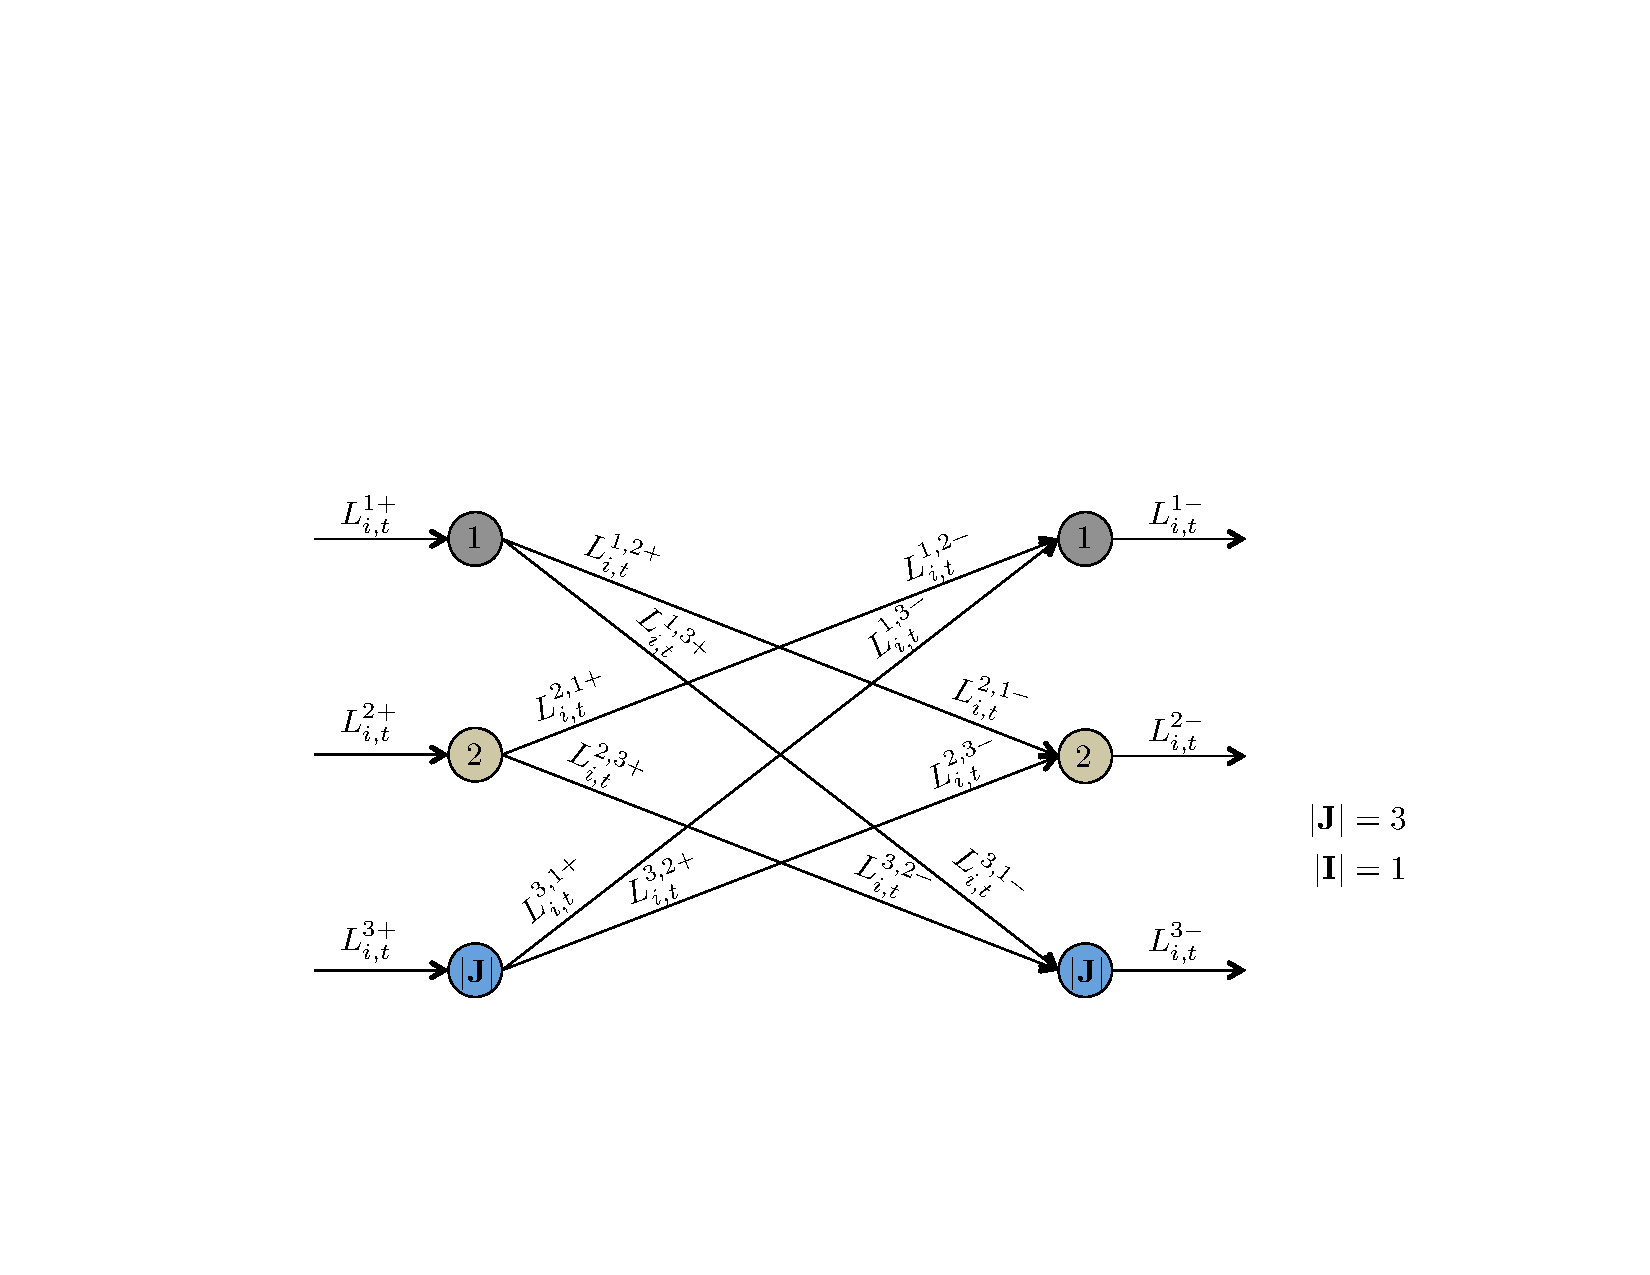
\includegraphics[trim=3cm 4cm 3cm 7cm, clip=true, totalheight=0.2\textheight]{Fig2.pdf}
\caption{A small instance of redistribution of product $i$ (and the only product)in time period $t$, represented by a flow diagram between three DCs}
\label{fig:redistribution_producti_all3DCs}
\end{figure}
In Figure \ref{fig:PDVRP_total12nodes}, we present the same network as shown in Figure \ref{fig:redistribution_producti_all3DCs}, adapted for PDVRP, where pickup and demand points are shown and aid our understanding of (\ref{eq:link}) and (\ref{eq:Fig3_2}).
\begin{figure}[H]
\centering
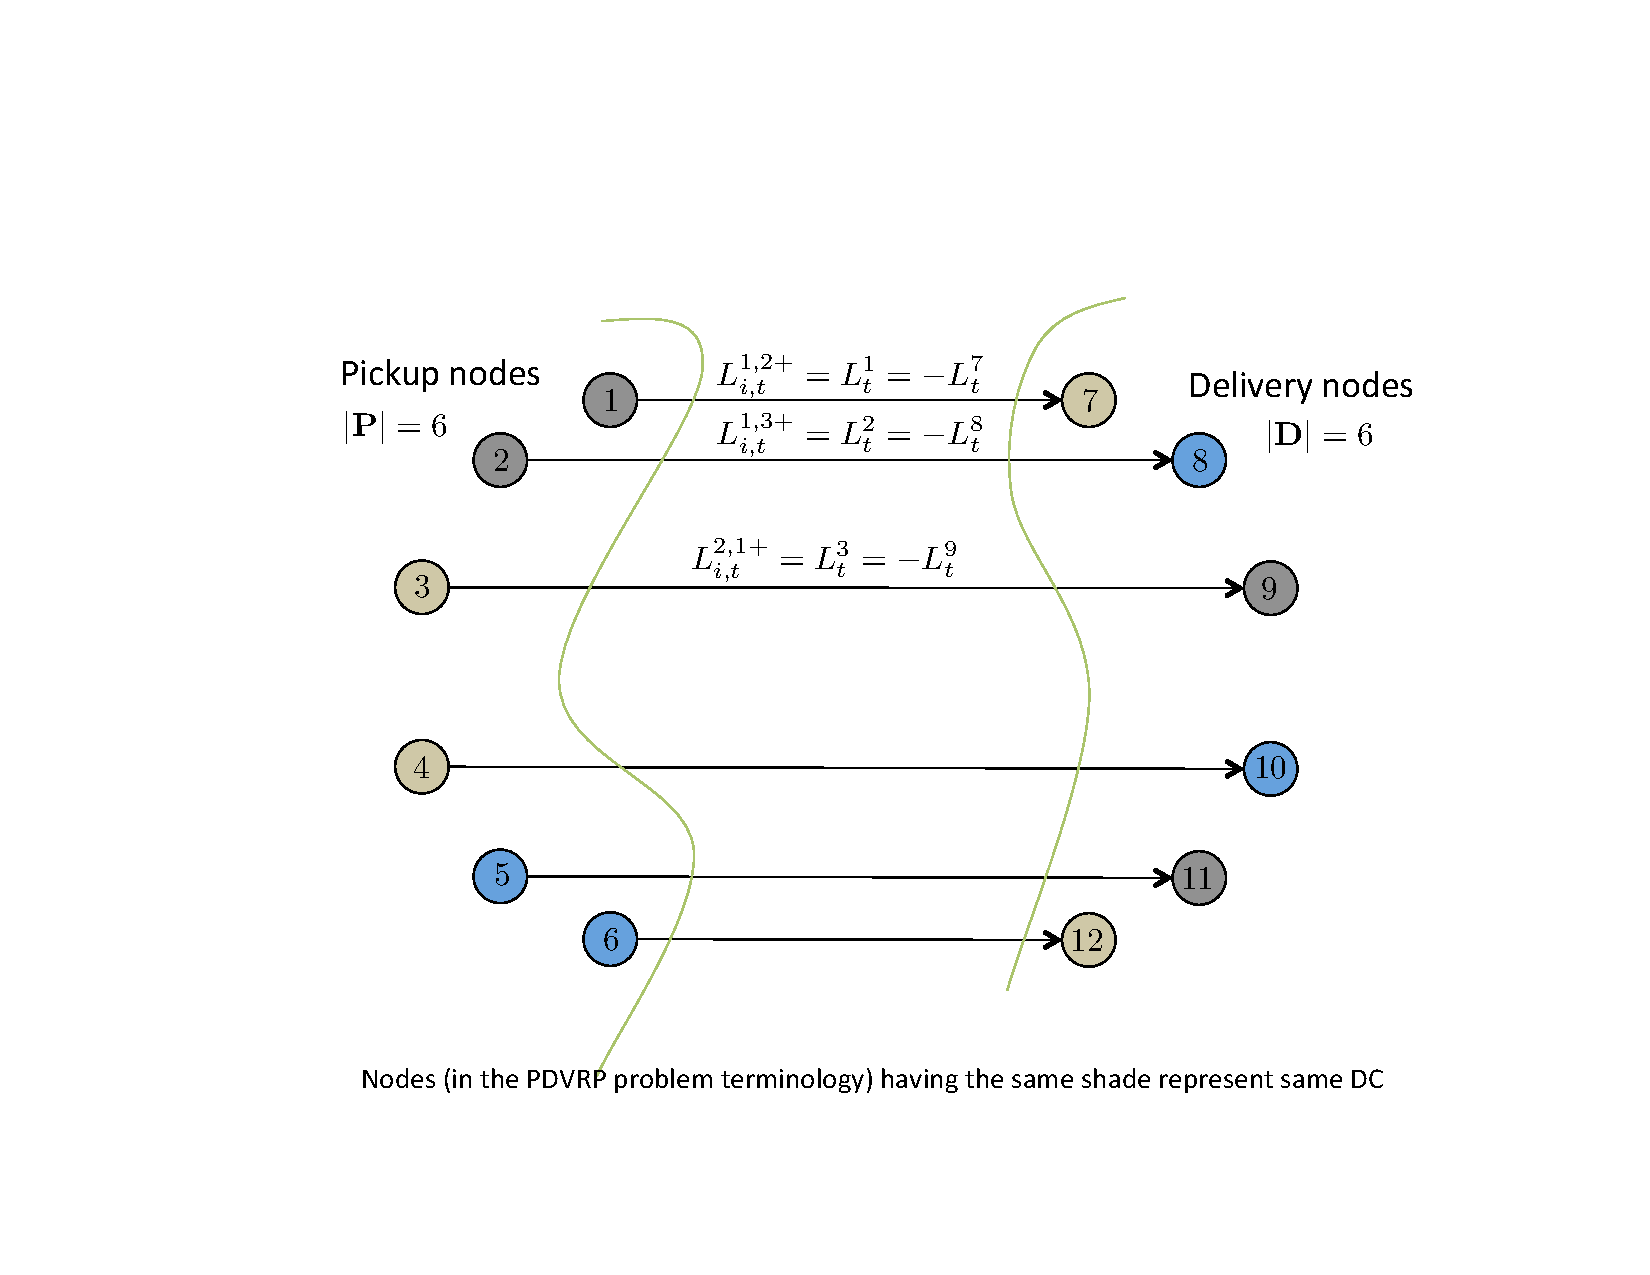
\includegraphics[trim=3cm 3cm 3cm 5cm, clip=true, totalheight=0.2\textheight]{Fig3.pdf}
\caption{An equivalent graph for the graph shown in Fig \ref{fig:redistribution_producti_all3DCs}, adapted for PDVRP problem}
\label{fig:PDVRP_total12nodes}
\end{figure}

Let us show how to linearize nonlinear "max" function with equality sign, in (\ref{eq:max1}) (rest of (\ref{eq:max2})-(\ref{eq:max4}) follow the same): \\
\begin{align}
D_{1,i,t}^{j} & = \max(D_{0,i,t}^{j}-d_{i,t}^{j},0) 
\qquad \qquad \qquad \qquad \qquad \nonumber \\
& \equiv
\left\{
\begin{matrix*}[l]
D_{1,i,t}^{j} & \geq & D_{0,i,t}^{j}-d_{i,t}^{j} \\
D_{1,i,t}^{j} & \geq & 0 \\
D_{1,i,t}^{j} & \leq & D_{0,i,t}^{j}-d_{i,t}^{j} + M (1-\lambda_{i,t}^{j}) \\
D_{1,i,t}^{j} & \leq & M \lambda_{i,t}^{j}\\
D_{0,i,t}^{j}-d_{i,t}^{j} & \leq & M \lambda_{i,t}^{j} \\
0 & \leq & D_{0,i,t}^{j}-d_{i,t}^{j} + M (1- \lambda_{i,t}^{j}) \\
\lambda_{i,t}^{j} & \in & \{0,1\}
\end{matrix*} \right.
\end{align}


Before we discuss the stochasticity in demands that we deal in our paper, let us first present a brief methodology for dealing with linear deterministic equivalent of stochastic programs. We refer the reader to \cite{Dantzig1993} for this. In the model \textbf{M1}, the demands $d_{i,t}^{j}, \forall (i,\bar{t},j)\in \textbf{ITJ}$, are deterministic, but our goal is to study the case when these are stochastic and spanning multiple time periods, and defined by individual demand scenarios. \\
Let us define sets $\textbf{SI}_{i,t}^{j}$ and $\textbf{ST}_{t}, \forall i\in \textbf{I}, j\in \textbf{J}, t=2,3,\ldots ,|\textbf{T}|$, containing scenarios for demands in individual case and that for collective case for each time period, respectively. \\
$\textbf{SI}_{i,t}^{j}=\{1,2,\ldots ,|\textbf{SI}_{i,t}^{j}|\}, \forall i\in \textbf{I}, j\in \textbf{J}, t=2,3,\ldots ,|\textbf{T}|$. Each scenario, $s_{i,t}^{j}\in \textbf{SI}_{i,t}^{j}$ is associated with a demand $d(s_{i,t}^{j})\geq 0$ (equivalent of $d_{i,t}^{j}$, for the stochastic case), with probability of occurrence $0<p(s_{i,t}^{j})\leq 1$, with $\sum_{s_{i,t}^{j}\in \textbf{SI}_{i,t}^{j}} p(s_{i,t}^{j})=1$. There can be two cases for $\textbf{SI}_{i,t}^{j}=\{1\}$, one, when the demand exists but is deterministic, and two, when there is no demand at all, i.e. $(i,t,j)\not \in \textbf{ITJ}$; in either case, we have $p(s_{i,t}^{j})=1$. \\
$\textbf{ST}_{t}=\{(x_{1},x_{2},\ldots,x_{|\textbf{I}||\textbf{J}|})|x_{|\textbf{J}|(i-1)+j}=s_{i,t}^{j}\in \textbf{SI}_{i,t}^{j}, \forall i\in \textbf{I},j\in \textbf{J}\}, \forall t=2,\ldots ,|\textbf{T}|$. An element of this set, $\omega_{t}=(x_{1},x_{2},\ldots,x_{|\textbf{I}||\textbf{J}|})\in \textbf{ST}_{t}$, represents a collective scenario for all demands in time period $t$. The probability associated with $\omega_t$ is $p(\omega_t)=\prod_{ij=1,\ldots ,|\textbf{I}||\textbf{J}|} p(x_{ij})$. The number of such scenarios in time period $t$ is given by $|\textbf{ST}_{t}|=\prod_{i\in \textbf{I},j\in \textbf{J}} |\textbf{SI}_{i,t}^{j}|, \forall t=2,\ldots ,|\textbf{T}|$. We will alternatively use $\tilde{\omega_t}$ to represent a random variable whose domain comes from the set $\textbf{ST}_t$, and each instance is the element $\omega_t\in \textbf{ST}_t$.\\

We break the time horizon in $|\textbf{T}|$ stages and reformulate model $\textbf{M1}$ for the deterministic equivalent of multistage "Stochastic Multi-Products Order-Redistribution Problem" with decisions in stage $t$ represented collectively by $y_t^{\tilde{\omega_t},\ldots ,\tilde{\omega_2}}, \forall t=2,\ldots ,|\textbf{T}|$ and by $y_1$ for $t=1$. We call this model as \textbf{M2}. Variables in stage 1 (i.e. $t=1$) are not scenario dependent, but for the rest of the stages, they are decided as per the realization of sequence of random variables ($\tilde{\omega_t},\ldots ,\tilde{\omega_2}$). Let us re-write all the variables that were mentioned earlier in model $\textbf{M1}$, which we now alternatively, and collectively refer to as $y_t^{\tilde{\omega_t},\ldots ,\tilde{\omega_2}}, \forall t=2,\ldots ,|\textbf{T}|$, or just, $y_t$: \\

$
\begin{matrix*}[l]
P_{i,\bar{t},t}^{j,(\tilde{\omega_t},\ldots ,\tilde{\omega_2})} & \forall (i,\bar{t},j)\in \textbf{ITJ}, \forall t \in \textbf{T}\\
Z_{\bar{t}}^{j,(\tilde{\omega_t},\ldots ,\tilde{\omega_2})} &  \forall (i,\bar{t},j)\in \textbf{ITJ}, \bar{t}=t\\
D_{1,i,t}^{j,(\tilde{\omega_t},\ldots ,\tilde{\omega_2})} &  \forall i \in \textbf{I}, \forall j \in \textbf{J}, \forall t \in \textbf{T}\\
D_{i,t}^{j{'},(\tilde{\omega_t},\ldots ,\tilde{\omega_2})}  & \forall i \in \textbf{I}, \forall j \in \textbf{J}, \forall t \in \textbf{T} \\
L_{i,t}^{j{+},(\tilde{\omega_t},\ldots ,\tilde{\omega_2})}  & \forall i \in \textbf{I}, \forall j \in \textbf{J}, \forall t \in \textbf{T} \\
U_{i,t}^{j{+},(\tilde{\omega_t},\ldots ,\tilde{\omega_2})} & \forall i \in \textbf{I}, \forall j \in \textbf{J}, \forall t \in \textbf{T} \\
D_{2,i,t}^{j,(\tilde{\omega_t},\ldots ,\tilde{\omega_2})} & \forall i \in \textbf{I}, \forall j \in \textbf{J}, \forall t \in \textbf{T} \\
L_{i,t}^{j{-},(\tilde{\omega_t},\ldots ,\tilde{\omega_2})} & \forall i \in \textbf{I}, \forall j \in \textbf{J}, \forall t \in \textbf{T} \\ 
U_{i,t}^{j{-},(\tilde{\omega_t},\ldots ,\tilde{\omega_2})} & \forall i \in \textbf{I}, \forall j \in \textbf{J}, \forall t \in \textbf{T} \\
D_{3,i,t}^{j,(\tilde{\omega_t},\ldots ,\tilde{\omega_2})} & \forall i \in \textbf{I}, \forall j \in \textbf{J}, \forall t \in \textbf{T} \\
D_{i,t}^{j{''},(\tilde{\omega_t},\ldots ,\tilde{\omega_2})} & \forall i \in \textbf{I}, \forall j \in \textbf{J}, \forall t \in \textbf{T} \\ 
S_{i,t}^{j,(\tilde{\omega_t},\ldots ,\tilde{\omega_2})} & \forall i \in \textbf{I}, \forall j \in \textbf{J}, \forall t \in \textbf{T} \qquad \text{(and so on)}\\
\end{matrix*}
$ \\
In addition to the above, $y$ variables will also include necessary slack variables to reduce all the stage $t$ constraints in the equality form as follows ($A_{t}$ and $B_{t-1}$ are the coefficient matrices and deterministic, whereas $b_t^{\tilde{\omega_t}}$ is the constant matrix which is dependent on scenario realization in stage $t$): \\
\[-B_{t-1} y_{t-1}^{\tilde{\omega_{t-1}},\ldots ,\tilde{\omega_2}} + A_{t} y_{t}^{\tilde{\omega_{t}},\ldots ,\tilde{\omega_2}}	= b_{t}^{\tilde{\omega_{t}}} \] \\
Now , we can write model \textbf{M2} with the new notation discussed above.\\ \\
MILP model, \textbf{M2}: \\
\begin{align*}
\text{min }z & = c_1 y_1 +E (c_2 y_2^{\tilde{\omega_2}} +\ldots + E (c_{|\textbf{T}|} y_{|\textbf{T}|}^{\tilde{\omega_{|\textbf{T}|}},\ldots ,\tilde{\omega_2}}) \ldots )
\end{align*}
\begin{align}
\begin{matrix}
A_1 y_1		& 									&													&	& = b_1\\
-B_{1} y_1	& + A_2 y_2^{\tilde{\omega_2}}		& 													& 	& = b_2^{\tilde{\omega_2}}\\
			& - B_{2} y_2^{\tilde{\omega_2}}	&+A_3 y_3^{\tilde{\omega_3},\tilde{\omega_2}}		& 	& = b_3^{\tilde{\omega_3}}\\
			& \ddots							& \ddots											&	& \vdots \\
			&									&-B_{|\textbf{T}|-1} y_{|\textbf{T}|-1}^{\tilde{\omega_{|\textbf{T}|-1}},\ldots ,\tilde{\omega_2}}	&+A_{|\textbf{T}|} y_{|\textbf{T}|}^{\tilde{\omega_{|\textbf{T}|}},\ldots ,\tilde{\omega_2}}	& = b_{|\textbf{T}|}^{\tilde{\omega_{|\textbf{T}|}}}
\end{matrix}
\end{align}
 
\pagebreak
\bibliographystyle{abbrv}
\begin{thebibliography}{10}
%APA style, replace "&" in authors with "and", and also give an emphasis on journal

\bibitem{Dantzig1993}
Dantzig, G. B., and Infanger, G. (1993). Multi-stage stochastic linear programs for portfolio optimization. \emph{Annals of Operations Research}, 45(1), 59-76.

\end{thebibliography}

\end{document}